% Created 2018-10-08 Mon 08:11
% Intended LaTeX compiler: pdflatex
\documentclass[presentation,9pt]{beamer}
\usepackage[utf8]{inputenc}
\usepackage[T1]{fontenc}
\usepackage{graphicx}
\usepackage{grffile}
\usepackage{longtable}
\usepackage{wrapfig}
\usepackage{rotating}
\usepackage[normalem]{ulem}
\usepackage{amsmath}
\usepackage{textcomp}
\usepackage{amssymb}
\usepackage{capt-of}
\usepackage{hyperref}
\usetheme{Hannover}
\author{Matheus Artur, Luís Alberto Cabús, Nicolas Leão, Fábio Vinícius}
\date{\url{https://github.com/projetosufal/data-structures-project}}
\title{Segment Tree}
\hypersetup{
 pdfauthor={Matheus Artur, Luís Alberto Cabús, Nicolas Leão, Fábio Vinícius},
 pdftitle={Segment Tree},
 pdfkeywords={},
 pdfsubject={},
 pdfcreator={Emacs 26.1 (Org mode 9.1.9)}, 
 pdflang={English}}
\begin{document}

\maketitle
\begin{frame}{Outline}
\tableofcontents
\end{frame}


\section{Intro}
\label{sec:org6c00d7c}

\begin{frame}[label={sec:org8eef74a}]{Stock Exchange}
\begin{columns}
\begin{column}{0.48\columnwidth}
\begin{block}{The problem}
\begin{itemize}
\item Data from thousands of companies worldwide, active for decades
\item Usage of multiple operations requiring da range/interval of time required
\item Efficiency demand
\end{itemize}
\end{block}
\end{column}

\begin{column}{0.48\columnwidth}
\begin{block}{O(n) operations?}
\begin{center}

\includegraphics[width=.9\linewidth]{./img/serv.png}
\end{center}
\end{block}
\end{column}
\end{columns}
\end{frame}
\section{Segment tree}
\label{sec:org6a430e8}
\begin{frame}[label={sec:org7e22879}]{Segment tree}
\begin{columns}
\begin{column}{0.48\columnwidth}
\begin{block}{How it is structured?}
\begin{itemize}
\item The Segtree is a binary tree that's represented from a array, where each node represents a unique interval or segment of the tree and stores a \alert{specific} value.
\item The value, is usually represented by \emph{maximum}, \emph{minimum} or \emph{sum} of the segment.
\end{itemize}
\end{block}
\end{column}
\begin{column}{0.48\columnwidth}
\begin{block}{Intervals of a A[6]}
\begin{center}
\begin{tabular}{lll}
\hline
tree[0] & = & A[0:5]\\
tree[1] & = & A[0:2]\\
tree[2] & = & A[3:5]\\
tree[3] & = & A[0:1]\\
tree[4] & = & A[2:2]\\
tree[5] & = & A[3:4]\\
tree[6] & = & A[5:5]\\
tree[7] & = & A[0:0]\\
tree[8] & = & A[1:1]\\
tree[9] & = & NULL\\
tree[10] & = & NULL\\
tree[11] & = & A[3:3]\\
tree[12] & = & A[4:4]\\
\hline
\end{tabular}
\end{center}
\end{block}
\end{column}
\end{columns}
\end{frame}
\begin{frame}[label={sec:org0a301bf}]{As tree}
\begin{center}
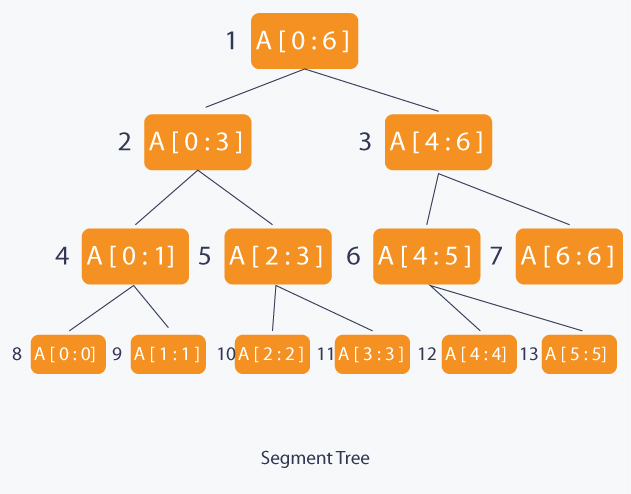
\includegraphics[width=.9\linewidth]{./img/segtree.jpg}
\end{center}
\end{frame}

\section{Operations}
\label{sec:org9315c9c}
\begin{frame}[label={sec:org191c94e}]{Operations}
\begin{block}{Building a tree}
\begin{itemize}
\item ( n log n) storage
\item but only (2*n - 1) actual nodes
\end{itemize}
\end{block}
\begin{block}{Query - range search}
\begin{itemize}
\item O(log n)
\end{itemize}
\end{block}
\begin{block}{Updating a tree}
\begin{itemize}
\item O(log n)
\item can modify any [l:r] section, than it will propagate updating dependencies
\end{itemize}
\end{block}
\end{frame}
\begin{frame}[fragile,label={sec:org5b4f4ac}]{Building a Segtree}
 \begin{verbatim}
void
buildtree(int (*f)(int l_num, int r_num), int *v, int *tree,
	  int *t_size, int node, int min, int max)
{
  int mid;
  
  if(min == max)
    tree[node] = v[min];

  else
    {
      mid = (min+max)/2;
      
      buildtree((*f), v, tree, t_size, 2*node + 1, min , mid);
      buildtree((*f), v, tree, t_size, 2*node + 2, mid + 1 , max);
      tree[node] = (*f)(tree[2*node +1], tree[2*node + 2]);
    }
}
\end{verbatim}
\end{frame}
\begin{frame}[fragile,label={sec:orgad4216a}]{Query}
 \begin{verbatim}
int
query(int (*f)(int l_num, int r_num), int *tree,
      int node, int min, int max, int l, int r)
{
  if(r < min || max < l)
    return 0;
  
  if(l <= min && max <= r)
    return tree[node];
  
  int mid, l_bipod, r_bipod;  
  mid = (min+max)/2;
  
  l_bipod = query((*f), tree, 2*node + 1, min , mid, l , r);
  r_bipod = query((*f), tree, 2*node + 2, mid + 1 , max, l, r);
  return((*f)(l_bipod, r_bipod));
}
\end{verbatim}
\end{frame}
\begin{frame}[fragile,label={sec:org2917607}]{Update}
 \begin{verbatim}
void
updatetree(int (*f)(int l_num, int r_num), int *tree,
	   int node, int min, int max, int l, int r, int val)
{
  int mid;
  if(min > max || min > r || max < l)
    return ;
  
  if(min == max)
    {
      tree[node] = val;
      return;
    }
  
  mid = (min+max)/2;
      
  updatetree((*f), tree, 2*node + 1, min , mid, l, r, val);
  updatetree((*f), tree, 2*node + 2, mid + 1 , max, l, r, val);
  
  tree[node] = (*f)(tree[2*node +1], tree[2*node + 2]);
}
\end{verbatim}
\end{frame}
\end{document}
